91. При приведённых условиях возможны всего 2 ситуации, изображённые ниже.
\begin{center}
\begin{figure}[ht!]
\center{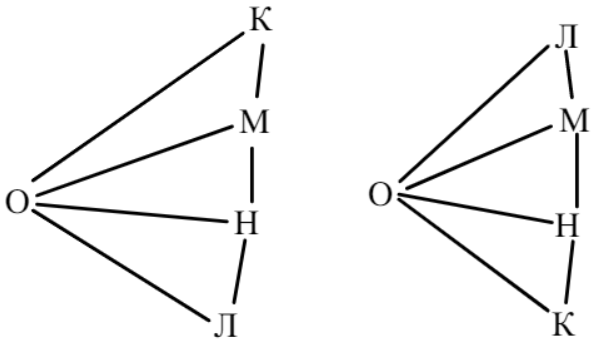
\includegraphics[scale=0.35]{dor2.png}}
\end{figure}
\end{center}
Как видно из картинки, выполняется утверждение Б. Отметим, что утверждение Г было бы верно, если бы из М можно было бы попасть {\bf только в один} из городов Н и О.\\
